\documentclass[11pt,a4paper]{article}

% ---------------------------------------------------------------------------
% Thermochemically consistent realization of a stochastic autocatalytic
% exporter: chemical completion, inherited operating certificates, cycle
% affinities and a necessary initiation scale.
%
% Author metadata: set the macros below before submission.  They are
% deliberately left blank in this version.  \CompanionAuthor is the author
% printed for the three companion manuscripts in refs.bib; \RepositoryNote
% is where the public repository location goes.
% ---------------------------------------------------------------------------
\newcommand{\PaperAuthor}{}
\newcommand{\PaperAffiliation}{}
\newcommand{\PaperDate}{14 September 2026}
\newcommand{\CompanionAuthor}{Anonymous}
\newcommand{\RepositoryNote}{The repository location will be supplied with the author information.}

\usepackage[T1]{fontenc}
\usepackage[utf8]{inputenc}
\usepackage{lmodern}
\usepackage{microtype}
\usepackage[a4paper,margin=1.05in]{geometry}
\usepackage{amsmath,amssymb,amsthm,mathtools}
\usepackage{booktabs}
\usepackage{array}
\usepackage{longtable}
\usepackage{enumitem}
\usepackage{xcolor}
\usepackage{graphicx}
\usepackage{tikz}
\usetikzlibrary{arrows.meta,positioning,calc}
\usepackage[obeyspaces,spaces]{url}
\usepackage[numbers,sort&compress]{natbib}
\usepackage[colorlinks=true,linkcolor=blue!55!black,citecolor=blue!55!black,urlcolor=blue!55!black]{hyperref}
\hypersetup{pdftitle={Thermochemically consistent realization of a stochastic autocatalytic exporter},
  pdfkeywords={autocatalysis, chemical reaction networks, stochastic thermodynamics, local detailed balance, chemostat, template replication, Lean}}

\DeclareUrlCommand\lean{\urlstyle{tt}}
\setlist{itemsep=2pt,topsep=3pt}
\setlength{\emergencystretch}{1.5em}
\graphicspath{{figures/}}

\theoremstyle{plain}
\newtheorem{theorem}{Theorem}[section]
\newtheorem{proposition}[theorem]{Proposition}
\newtheorem{lemma}[theorem]{Lemma}
\newtheorem{corollary}[theorem]{Corollary}
\theoremstyle{definition}
\newtheorem{definition}[theorem]{Definition}
\theoremstyle{remark}
\newtheorem{remark}[theorem]{Remark}

\newcommand{\E}{\mathbb E}
\newcommand{\Prob}{\mathbb P}
\newcommand{\N}{\mathbb N}
\newcommand{\R}{\mathbb R}
\newcommand{\Z}{\mathbb Z}
\newcommand{\eps}{\varepsilon}
\newcommand{\dd}{\,\mathrm d}
\newcommand{\Sint}{S_{\mathrm{int}}}
\newcommand{\Sfull}{S_{\mathrm{full}}}
\newcommand{\cP}{c_{\mathrm p}}
\newcommand{\cD}{c_{\mathrm d}}
\newcommand{\Good}{G_{V,H}}
\newcommand{\Bud}{\mathcal B}
\newcommand{\cE}{c_{\mathrm E}}
\newcommand{\cW}{c_{\mathrm W}}
\newcommand{\EE}{E_{\mathrm E}}
\newcommand{\ER}{E_{\mathrm R}}
\newcommand{\EY}{E_{\mathrm Y}}
\newcommand{\ES}{E_{\mathrm S}}
\newcommand{\tseed}{\tau_{\mathrm{seed}}}
\newcommand{\aseed}{a_{\mathrm{seed}}}
\newcommand{\GV}{\mathcal G_V}
\newcommand{\Aff}{\mathcal A}

\title{Thermochemically consistent realization of a\\ stochastic autocatalytic exporter:\\[4pt]
\large chemical completion, inherited operating certificates, cycle affinities and a necessary initiation scale}
\author{\PaperAuthor\\ \small \PaperAffiliation}
\date{\PaperDate}

\begin{document}
\maketitle

\begin{abstract}
A quantitative stochastic reaction model is physically informative only if its chemical completion preserves the propensities and the meaning of its output and resource counters. We exhibit such a completion for a maintained autocatalytic exporter whose finite-time operating, output and supply guarantees were proved in a companion paper as statements about a twenty-channel labelled count process. Six reversible chemical pairs on eight species admit positive elemental compositions and a single standard-potential assignment throughout a two-parameter rectangle of paired release and cleavage speeds; at unit fuel and waste activities their mass-action count propensities, stoichiometric updates, export marks and service marks coincide label by label with the certified source. Consequently every inherited estimate transfers without a change of constants: outward interval evaluation of the proved error budget gives success probabilities of at least $0.923849$, $0.994201$ and $0.999558$ for one hundred observation windows at copy scales $10^8$, $2\times10^8$ and $3\times10^8$, while deleting only the templated ligation pair, with every other chemical specification retained, bounds the probability of the same output schedule below $10^{-21699}$ at the first scale. We then extract three consequences of the completed chemistry. The internal stoichiometric cycles are exactly a passive cycle of zero affinity and one emergent fuel-to-waste cycle of affinity $\log(8\times10^{10})$; local detailed balance holds for the count propensities at neighbouring states with the falling-factorial convention; and, because the preparation contains food only, the first template can arise only through two channels, which yields the necessary initiation bound $V\ge(4\times10^8/401)\log(1/\eps_0)$ for any operating guarantee with failure probability at most $\eps_0$, about $4.59\times10^6$ at $99\%$. Dimensional examples make the eight-hour startup allowance, the gross chemical service and the mixed-species character of the exported product explicit, and a conditional stock-sizing relation delimits the remaining extension to autonomous finite reservoirs. The algebraic and finite marked-kernel statements are verified in Lean~4; the identification with a nonexplosive count process and the initiation argument are conventional proofs, and every printed decimal is an interval-certified evaluation of a proved bound rather than a simulation.
\end{abstract}

\section{Introduction}\label{sec:intro}

Structural theories of autocatalysis, from Kauffman's autocatalytic sets~\citep{kauffman1986} through the RAF formalism~\citep{hordijk2004,steel2019} to the stoichiometric classification of autocatalytic cores~\citep{blokhuis2020}, certify that a network can in principle make its own catalysts from a food source, and experimental template replicators~\citep{vonkiedrowski1986,sievers1994,lincoln2009} and kinetic design principles for minimal autocatalysts~\citep{sakref2024} show what such mechanisms look like chemically. A different kind of statement is an \emph{operating certificate}: a proved lower bound on the probability that an explicit finite-copy stochastic reactor, prepared with food alone, establishes catalytic material by a deadline, keeps it against washout and active destruction, and exports a prescribed amount of product in every observation window for a prescribed duration, within stated allowances of food and external driving. A companion paper~\citep{exporter2026} proves such a certificate for a six-species template reactor with a maintained-drive cleavage competitor, as a theorem about a twenty-channel labelled Markov jump process with mass-action propensities, and sharpens an earlier fixed-horizon result~\citep{finitecopy2026}.

Such a theorem is stated for a labelled generator with effective rate coefficients. Whether that generator is the count process of \emph{some} balanced chemistry with fixed standard potentials, maintained reservoirs and a consistent identical-reactant convention is a separate question, and it can fail in at least three ways. Reservoir species omitted from the generator can make two effective pairs demand incompatible equilibrium ratios, so that no single potential assignment exists. A different convention for a reaction between identical molecules, $2X\rightleftharpoons Z$ here, changes the propensity and hence the generator. And resource or output counters that are attached only after the dynamics has been projected to concentrations can lose the joint event whose probability is being certified. Open-network thermodynamics~\citep{polettini2014,rao2016,rao2018,falasco2025} and the stochastic thermodynamics of reaction networks~\citep{schmiedl2007} say what a consistent completion must look like: elemental balance, a potential assignment satisfying local detailed balance, chemostatted species whose maintenance carries the affinity of emergent cycles. The question addressed here is whether the certified exporter admits such a completion \emph{exactly}, with the same propensities, marks and preparation, so that the inherited probability bounds become statements about a specified open chemical model rather than about an abstract source.

\paragraph{Contributions.}
The answer is affirmative, and the completion has consequences of its own.
\begin{enumerate}[label=(\roman*)]
\item \emph{Realization} (Theorem~\ref{thm:realization}). Six reversible pairs on the species $U,W,X,C_1,C_2,Z,F,P$, with $F,P$ maintained fuel and waste, balance three neutral elemental components and admit one standard-potential assignment, independent of the release speed $r\in[19,21]$ and the cleavage speed $\delta\in[1/50,1/25]$. At unit reservoir activities their count propensities, updates, export marks and service marks equal the certified source with ligation bias $K=10$, label by label, including the falling-factorial convention for $2X\rightleftharpoons Z$.
\item \emph{Transfer} (Theorem~\ref{thm:transfer}, Proposition~\ref{prop:disabled}). The companion's finite-duration error budget, its simple exponential bound, its output and service corollaries, and its matched-deletion comparison hold verbatim for the completed model. Deleting only $C_2\rightleftharpoons Z$ preserves elemental balance, thermochemistry, the competing driven pair, the preparation and the observation protocol, so the comparison is between two consistently specified chemistries meeting the same output requirement.
\item \emph{Cycle structure and count-level local detailed balance} (Section~\ref{sec:cycles}). The kernel of the internal stoichiometric matrix is spanned by a passive cycle and a drive cycle; the full matrix kills only the passive one and sends the drive cycle to $e_P-e_F$. The affinity of $a\cP+b\cD$ is $b\log(8\times10^{10})$, so the six-pair subnetwork has exactly one independent fuel/waste driving direction. The forward and reverse propensities at neighbouring count states satisfy local detailed balance with an explicit count-level potential.
\item \emph{A necessary initiation scale} (Theorem~\ref{thm:init}). Starting from food only, the first template is created by basal ligation or by the reverse driven channel, with combined coefficient $\alpha_\delta$. A reference immigration--death construction and Jensen's inequality give $\Prob(\tseed>t)\ge e^{-\alpha_\delta Vt}$, hence any guarantee of the operating event with failure at most $\eps_0$ requires $V\ge\log(1/\eps_0)/(500\alpha_\delta)\ge(4\times10^8/401)\log(1/\eps_0)$. Sufficient and necessary copy scales are therefore both logarithmic in the confidence, with a factor of about $39$ between the exponent coefficients.
\item \emph{Physical accounting and scope} (Sections~\ref{sec:units}--\ref{sec:resident}). A dimensional reading at $1$~mM and a one-minute time unit gives sub-picolitre volumes, an $8$~h~$20$~min startup allowance, whole-run food and driving allowances, a bound of about $0.775$~nJ on the chemical work of the fuel/waste pair, and a mixed-species product. A proved activity corridor and conditional stock-sizing relation state precisely what a finite fuel/waste bath would additionally require, and a companion resident completion shows the same bookkeeping principle in a compartment model.
\end{enumerate}

\paragraph{Verification and the three kinds of evidence.}
Three kinds of statement appear and are kept apart throughout. The algebraic identities (balance, potentials, coefficient binding, source projection, cycle classification, neighbouring-count ratios, initiation algebra, activity bounds) and the finite marked-kernel probability inequalities are verified in Lean~4~\citep{demoura2021} with Mathlib~\citep{mathlib2020}; Appendix~\ref{app:formal} maps every such claim to a declaration and records the verification receipts. The identification of the finite stopped construction with the literal infinite-state count process, and the reference-process construction of Theorem~\ref{thm:init}, are conventional proofs written out in full (Appendix~\ref{app:process} and Section~\ref{sec:init}). Every printed decimal is an evaluation of a proved bound in outward-rounded interval arithmetic; no trajectory is simulated anywhere in the paper.

\paragraph{What is not claimed.}
The model is schematic chemistry: three formal neutral elemental components, ideal activities in the sense of~\citep{rao2016,avanzini2021}, and effective reactions, one of which, the reverse driven channel $U+W+P\to X+F$, is trimolecular and is not asserted to be elementary. No laboratory molecule is identified, no rate is fitted, and the maintained reservoirs are activities, not finite stocks. Varying $r$ and $\delta$ changes both directions of a pair together and preserves every equilibrium ratio; nothing is claimed about robustness to independent changes of individual rate constants. The deletion comparison attributes the certified output schedule to the templated cycle within two specified generators; it does not prove that fuel consumption is necessary for export. The necessary initiation bound is necessary, not sufficient, and neither it nor the sufficient rule is claimed optimal in the observation duration. Finally, the probability estimates are inherited: the contribution is their exact chemical realization and its consequences, and the paper credits them accordingly.

\paragraph{Organization.}
Section~\ref{sec:model} specifies the completed chemistry, the environment, the preparation and the observation protocol. Section~\ref{sec:realization} proves the realization theorem. Section~\ref{sec:transfer} states the inherited guarantee, its consequences and the deletion comparison. Section~\ref{sec:cycles} classifies cycles and proves count-level local detailed balance. Section~\ref{sec:init} proves the necessary initiation scale. Section~\ref{sec:units} gives the dimensional example, Section~\ref{sec:bath} the finite-reservoir relation, Section~\ref{sec:resident} the resident companion, and Section~\ref{sec:discussion} discusses scope and open questions. Appendix~\ref{app:process} contains the conventional process identification and Appendix~\ref{app:formal} the formal evidence.

\section{The completed chemical model}\label{sec:model}

\subsection{Species, pairs and coefficients}\label{sec:pairs}
The internal species, in order, are $U,W,X,C_1,C_2,Z$: two foods, the covalent product and template $X=UW$, the two substrate-binding complexes $C_1=X{:}U$ and $C_2=X{:}(U,W)$, and the duplex $Z=X{:}X$. Two further species, a fuel $F$ and a waste $P$, are maintained at fixed activities $a_F,a_P$. Write
\begin{equation}\label{eq:parameters}
 \eps=\frac1{500\,000\,000},\qquad \eta=\frac1{8\,000\,000\,000},\qquad
 (r,\delta)\in[19,21]\times\Big[\frac1{50},\frac1{25}\Big].
\end{equation}
Table~\ref{tab:chem} lists the six reversible chemical pairs with their normalized mass-action coefficients; concentrations and time are dimensionless until Section~\ref{sec:units}. For copy scale $V\in\N_{>0}$ and counts $n=(u,w,x,c_1,c_2,z)\in\N^6$ the forward and reverse count propensities of the pairs are
\begin{equation}\label{eq:propensities}
\begin{aligned}
 a^+&=\Big(\eps\frac{uw}{V},\;20\frac{xu}{V},\;20\frac{c_1w}{V},\;20c_2,\;rz,\;\delta a_F\,x\Big),\\
 a^-&=\Big(\frac{\eps x}{10},\;20c_1,\;20c_2,\;2z,\;r\frac{x(x-1)}{V},\;\delta\eta\,a_P\frac{uw}{V}\Big).
\end{aligned}
\end{equation}
The identical-reactant propensity of $2X\to Z$ is the falling factorial $x(x-1)/V$ with no additional factor $1/2$; this convention is the one under which the potential assignment of Section~\ref{sec:realization} closes at the count level (Proposition~\ref{prop:ldb}). The reverse driven reaction $U+W+P\to X+F$ has three reactant species; it is an effective channel of the model, and an elementary implementation is not asserted.

\begin{table}[t]
\centering
\caption{The completed reversible chemical subnetwork. The forward orientation fixes all stoichiometric signs. Labels refer to the twenty-channel source of Table~\ref{tab:source}. The parameters $r$ and $\delta$ multiply both directions of their pair, so every ratio $k_j^+/k_j^-$ is fixed.}\label{tab:chem}
\begin{tabular}{cllccc}
\toprule Pair & Reaction & Labels & $k_j^+$ & $k_j^-$ & $k_j^+/k_j^-$\\\midrule
0 & $U+W\rightleftharpoons X$ & 0, 1 & $\eps$ & $\eps/10$ & $10$\\
1 & $X+U\rightleftharpoons C_1$ & 2, 3 & $20$ & $20$ & $1$\\
2 & $C_1+W\rightleftharpoons C_2$ & 4, 5 & $20$ & $20$ & $1$\\
3 & $C_2\rightleftharpoons Z$ & 6, 7 & $20$ & $2$ & $10$\\
4 & $Z\rightleftharpoons 2X$ & 8, 9 & $r$ & $r$ & $1$\\
5 & $X+F\rightleftharpoons U+W+P$ & 18, 19 & $\delta$ & $\delta\eta$ & $8\times10^{9}$\\\bottomrule
\end{tabular}
\end{table}

\subsection{Environment, preparation and labels}\label{sec:environment}
Eight further labelled operations describe the environment: separate feeds of $U$ and $W$, each a Poisson stream of rate $V$, and washout of each internal species at rate equal to its count. Feed and washout are transfers between the reactor and external inventory; they are not reactions to or from an empty complex, and no thermodynamic reversibility is asserted for them. Together with the twelve chemical directions this gives the twenty labels of Table~\ref{tab:source}, numbered as in the companion paper so that pair 3 occupies labels 6 and 7 and the two driven directions are the distinct labels 18 and 19. The preparation is always the food-only state $n_0=(V,V,0,0,0,0)$. Time is dimensionless with unit dilution rate; $V$ divides every bimolecular propensity and equals each feed rate, so that $n/V$ obeys the classical density scaling~\citep{kurtz1972,anderson2015}. Figure~\ref{fig:network} shows the mechanism and its external services.

\begin{table}[t]
\centering\small
\caption{The twenty-channel labelled source at unit reservoir activities. A mark is the increment of the indicated cumulative counter; every unlisted mark is zero. Channels $6$ and $7$ are the only channels removed in the deletion comparison of Section~\ref{sec:disabled}. Channels $18$ and $19$ change the six counts exactly as channels $1$ and $0$ but carry distinct service marks and a different coefficient ratio.}\label{tab:source}
\begin{tabular}{rllcc}
\toprule Label & Transition & Propensity & Export mark & Service mark $(Q_F,Q_P)$\\\midrule
0 & $U+W\to X$ & $\eps uw/V$ & & \\
1 & $X\to U+W$ & $\eps x/10$ & & \\
2 & $X+U\to C_1$ & $20xu/V$ & & \\
3 & $C_1\to X+U$ & $20c_1$ & & \\
4 & $C_1+W\to C_2$ & $20c_1w/V$ & & \\
5 & $C_2\to C_1+W$ & $20c_2$ & & \\
6 & $C_2\to Z$ & $20c_2$ & & \\
7 & $Z\to C_2$ & $2z$ & & \\
8 & $Z\to 2X$ & $rz$ & & \\
9 & $2X\to Z$ & $rx(x-1)/V$ & & \\
10, 11 & feed of $U$; feed of $W$ & $V$; $V$ & & \\
12, 13 & washout of $U$; of $W$ & $u$; $w$ & $0$; $0$ & \\
14, 15 & washout of $X$; of $C_1$ & $x$; $c_1$ & $4$; $4$ & \\
16, 17 & washout of $C_2$; of $Z$ & $c_2$; $z$ & $4$; $8$ & \\
18 & $X+F\to U+W+P$ & $\delta x$ & & $(1,0)$\\
19 & $U+W+P\to X+F$ & $\delta\eta uw/V$ & & $(0,1)$\\\bottomrule
\end{tabular}
\end{table}

\begin{figure}[t]
\centering
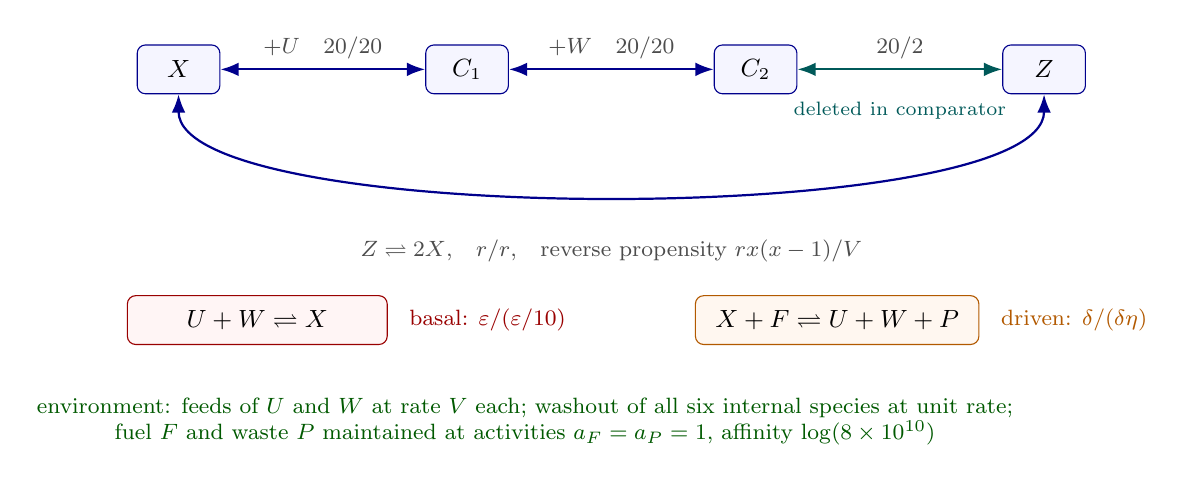
\begin{tikzpicture}[>=Latex,node distance=2.6cm,
  sp/.style={draw=blue!55!black,rounded corners=3pt,fill=blue!4,minimum width=1.05cm,minimum height=.62cm,font=\small},
  lab/.style={font=\footnotesize,text=black!70},
  env/.style={font=\footnotesize,text=green!35!black}]
\node[sp] (X) {$X$};
\node[sp,right=of X] (C1) {$C_1$};
\node[sp,right=of C1] (C2) {$C_2$};
\node[sp,right=of C2] (Z) {$Z$};
\draw[<->,thick,blue!55!black] (X) -- node[lab,above]{$+U$\quad $20/20$} (C1);
\draw[<->,thick,blue!55!black] (C1) -- node[lab,above]{$+W$\quad $20/20$} (C2);
\draw[<->,thick,teal!70!black] (C2) -- node[lab,above]{$20/2$} node[lab,below,yshift=-8pt,font=\scriptsize,text=teal!70!black]{deleted in comparator} (Z);
\draw[<->,thick,blue!55!black] (Z.south) .. controls ($(Z.south)+(0,-1.7)$) and ($(X.south)+(0,-1.7)$) .. (X.south);
\node[lab,anchor=north] at ($(X.south)!0.5!(Z.south)+(0,-1.72)$) {$Z\rightleftharpoons 2X$,\quad $r/r$,\quad reverse propensity $rx(x-1)/V$};
\node[sp,fill=red!4,draw=red!60!black,below=2.55cm of X,xshift=1.0cm,minimum width=3.3cm] (basal) {$U+W\rightleftharpoons X$};
\node[lab,text=red!60!black,right=.15cm of basal] {basal: $\eps/(\eps/10)$};
\node[sp,fill=orange!6,draw=orange!70!black,right=3.9cm of basal,minimum width=3.6cm] (drive) {$X+F\rightleftharpoons U+W+P$};
\node[lab,text=orange!70!black,right=.15cm of drive] {driven: $\delta/(\delta\eta)$};
\node[env,below=.55cm of basal,xshift=3.4cm,align=center] {environment: feeds of $U$ and $W$ at rate $V$ each; washout of all six internal species at unit rate;\\ fuel $F$ and waste $P$ maintained at activities $a_F=a_P=1$, affinity $\log(8\times10^{10})$};
\end{tikzpicture}
\caption{The completed source and its external services. Arrow annotations give forward/reverse normalized coefficients. The catalytic route $X\to C_1\to C_2\to Z\to 2X$ has net reaction $U+W\to X$ with the initiating template returned; the basal pair performs the same net reaction without a template. The driven forward reaction consumes fuel while cleaving $X$; its reverse creates $X$ from the two foods and the waste. Washout of template-containing species supplies the measured export.}\label{fig:network}
\end{figure}

\subsection{Observables and the operating event}\label{sec:event}
Define the two food moieties, the weighted catalytic count and the covalent stock by
\begin{equation}\label{eq:observables}
 A=u+x+2c_1+2c_2+2z,\qquad B=w+x+c_1+2c_2+2z,\qquad
 Y=x+\tfrac98c_1+\tfrac75c_2+\tfrac95z .
\end{equation}
Every chemical channel, including both driven directions, preserves $A$ and $B$; only feeds and washouts change them. Let $E(t)$ be the cumulative export with the marks of Table~\ref{tab:source}, so that $E/4$ counts \emph{template equivalents} leaving the reactor in free product, in complexes and in duplexes; the marks do not separate free $X$ from exported complexes. Let $I_U,I_W$ count the two feeds and $Q_F,Q_P$ the two driven directions; $Q_D=Q_F+Q_P$ is the \emph{gross} driving service. Fix a post-startup duration $H=m+s$ with $m\in\N$ complete unit windows and a final fraction $0\le s<1$, and put $T=500+H$.

\begin{definition}[Operating event]\label{def:event}
The event $\Good$ consists of the following simultaneous requirements.
\begin{enumerate}[label=(\alph*)]
\item \emph{Resources:} $A(t),B(t)\in[0.9V,1.1V]$ for all $t\le T$.
\item \emph{Entry and residence:} $Y$ reaches $V/2500$ by time $500$ and never subsequently reaches $Y\le V/5000$ before $T$.
\item \emph{Output:} on every complete window $[500+i,501+i]$, $0\le i<m$, the export increment is at least $V/5000$ marks, i.e.\ $V/20000$ template equivalents.
\item \emph{Supplies:} over $[0,T]$, $I_U,I_W\le2VT$ and $Q_D\le VT/8$.
\end{enumerate}
\end{definition}
Window boundaries reset only the measurement counter; the chemical state, the entry/residence phase and all cumulative counters persist. The success event is a joint event of one law, not a conjunction of separately estimated marginals; the identification of the finite marked construction with this event on the literal count process is the subject of Appendix~\ref{app:process}.

\section{Material balance, thermochemistry and the marked-source identity}\label{sec:realization}

Assign the eight species the composition vectors, in three formal neutral elemental units,
\begin{equation}\label{eq:composition}
 U{:}(1,0,0),\ W{:}(0,1,0),\ X{:}(1,1,0),\ C_1{:}(2,1,0),\ C_2{:}(2,2,0),\ Z{:}(2,2,0),\ F{:}(0,0,1),\ P{:}(0,0,1),
\end{equation}
and, in units of $RT$, the standard chemical potentials
\begin{equation}\label{eq:potential}
 g=\big(0,\;0,\;-\log10,\;-\log10,\;-\log10,\;-2\log10,\;\log10+\log(8\times10^{9}),\;0\big).
\end{equation}
Let $\nu_j\in\Z^8$ be the product-minus-reactant column of pair $j$ and let $\Sfull=(\nu_0,\dots,\nu_5)$; let $\Sint$ be its restriction to the six internal rows.

\begin{theorem}[Realization]\label{thm:realization}
For every $(r,\delta)\in[19,21]\times[1/50,1/25]$ the completed chemistry of Section~\ref{sec:model} has the following properties.
\begin{enumerate}[label=(\alph*)]
\item \emph{Balance.} Every pair conserves each of the three elemental components of~\eqref{eq:composition}, and all charges are zero.
\item \emph{Common thermochemistry.} All twelve coefficients are positive and
\begin{equation}\label{eq:thermo}
 \log\frac{k_j^+}{k_j^-}=-\nu_j\cdot g\qquad(j=0,\dots,5),
\end{equation}
with the single assignment~\eqref{eq:potential}, independent of $r,\delta$. The fuel/waste potential difference is $g_F-g_P=\log(8\times10^{10})$.
\item \emph{Coefficient binding.} For every count vector, copy scale and activities $a_F,a_P$, the propensity of each direction equals its coefficient times the mass-action substrate factor of the displayed complex, with the falling factorial $x(x-1)/V$ for $2X\to Z$ and the activity factors $a_F$, $a_P$ multiplying only the driven directions.
\item \emph{Marked-source identity.} At $a_F=a_P=1$ the twenty labelled count propensities, the stoichiometric updates, the export marks and the two service marks coincide label by label with the companion source at ligation bias $K=10$ and the same $(r,\delta)$.
\item \emph{Family.} The rectangle $[19,21]\times[1/50,1/25]$ is compact with nonempty interior, contains the rational point $(20,3/100)$, and is contained in the companion box $K\in[8,12]$, $r\in[18,22]$, $\delta\in[1/100,1/20]$.
\end{enumerate}
\end{theorem}

\begin{proof}
(a) Each row of Table~\ref{tab:chem} is checked directly against~\eqref{eq:composition}: for instance $C_2\to Z$ maps $(2,2,0)$ to $(2,2,0)$, $Z\to2X$ maps $(2,2,0)$ to $2(1,1,0)$, and $X+F\to U+W+P$ maps $(1,1,0)+(0,0,1)$ to $(1,0,0)+(0,1,0)+(0,0,1)$. Reverse directions balance by symmetry.

(b) Positivity is immediate from $r,\delta>0$. Substituting~\eqref{eq:potential}: for pair 0, $-\nu_0\cdot g=g_U+g_W-g_X=\log10=\log(\eps/(\eps/10))$; for pairs 1 and 2, $g_X+g_U-g_{C_1}=0$ and $g_{C_1}+g_W-g_{C_2}=0$; for pair 3, $g_{C_2}-g_Z=\log10=\log(20/2)$; for pair 4, $g_Z-2g_X=0=\log(r/r)$; for pair 5, $g_X+g_F-g_U-g_W-g_P=-\log10+\log10+\log(8\times10^9)=\log(1/\eta)=\log(\delta/(\delta\eta))$. The release and cleavage speeds cancel in their ratios, so the assignment does not depend on $(r,\delta)$.

(c) is the definition~\eqref{eq:propensities} read direction by direction; the point of stating it is that the thermochemistry of (b) is attached to the very coefficients that multiply the count substrate factors, not to an unrelated rate array.

(d) The companion source with parameters $(\eps,k,r,\delta)$ has basal reverse coefficient $\eps k$ with $k=K^{-1}$, templated reverse coefficient $20k$ for $Z\to C_2$, duplex association $rx(x-1)/V$, driven coefficients $\delta$ and $\delta\eta$ with $\eta=\eps/16$, feeds $V$, washouts equal to counts, export marks $(0,0,4,4,4,8)$ on the six washouts and unit service marks on the two driven labels. At $K=10$ these are exactly~\eqref{eq:propensities} at unit activities and Table~\ref{tab:source}; the reactant and product complexes of every direction, projected to the internal species, are the companion's arrays, so the natural-count updates agree. Note that the companion's low-level parameter is $k=1/K$; using $k=10$ would be a source error.

(e) is arithmetic. The formal statements are \lean{material_balance}, \lean{common_thermochemistry}, \lean{coefficient_binding}, \lean{rate_projection}, \lean{marked_projection} and \lean{rectangle_compact} (Appendix~\ref{app:formal}).
\end{proof}

\begin{remark}[Paired variation is not rate robustness]\label{rem:paired}
Because $r$ and $\delta$ scale both directions of their pairs, every point of the rectangle has the same equilibrium ratios and the same potentials. The rectangle is therefore a family of \emph{kinetic} realizations of one thermochemistry. Nothing is claimed for perturbations that change $k_j^+$ and $k_j^-$ independently; in particular, a change of the driven ratio $\eta a_P/a_F$ by varying reservoir activities is a change of thermochemistry and is treated separately in Section~\ref{sec:bath}.
\end{remark}

\begin{remark}[A productive interior state]\label{rem:productive}
The rectangle is not an arbitrary sub-box of the companion's. At the concentration state $x=10^{-4}$, $c_1=\tfrac35x$, $c_2=\tfrac3{10}x$, $z=\tfrac6{25}x$ with unit food concentrations, the four catalytic drift components of the deterministic rate law, including washout and both driven directions, are affine in $(r,\delta)$ and bounded below on the whole rectangle by $381100249/(5\times10^{13})$, $7/50000$, $9/500000$ and $2421/10^8$, all positive (\lean{productive_positive}). The $x$-component changes sign at $\delta^*=581099999/4999993750\approx0.11622$ for $r=19$ and is negative at $\delta=1/5$ (\lean{productive_boundary_failure}). This instantaneous witness is separate from the food-only preparation and is not an inoculum; it only illustrates that the admitted cleavage interval sits well inside the region where the mechanism is productive at this composition.
\end{remark}

\section{The inherited operating guarantee and matched deletion}\label{sec:transfer}

\subsection{The finite-duration error budget}\label{sec:budget}
Define the constants and error terms of the companion's finite-duration theorem,
\begin{equation}\label{eq:constants}
 \cE=\frac{8047}{312\,500\,000\,000},\qquad \cW=\frac{13}{1\,080\,000},
\end{equation}
\begin{equation}\label{eq:terms}
\begin{aligned}
 \EE(V)&=e^{-\cE V}+e^{-3V/500},\\
 \ER(V,T)&=4e^{-V/1000}+12000\,VT\,e^{1/50-V/2000},\\
 \EY(V,T)&=e^{-V/62500}+3000\,VT\,e^{18/125-V/15625},\\
 \ES(V,T)&=2e^{-(2\log2-1)VT}+e^{-VT/200},
\end{aligned}
\end{equation}
\begin{equation}\label{eq:budget}
 \Bud(V,H)=\EE(V)+\ER(V,T)+\EY(V,T)+m\,e^{1/8-\cW V}+\ES(V,T),\qquad T=500+H,\ m=\lfloor H\rfloor .
\end{equation}
The five groups bound, respectively, missed entry, resource exit, loss of residence, failure of some window, and violation of a supply budget. All terms are retained even when numerically negligible.

\begin{theorem}[Transfer of the operating guarantee]\label{thm:transfer}
For every $(r,\delta)$ in the rectangle, every positive integer $V$ and every $H\ge0$, the finite marked law of the completed source satisfies
\begin{equation}\label{eq:success}
 \Prob(\Good)\ge\max\{0,\,1-\Bud(V,H)\},
\end{equation}
and if moreover $V\ge10^8$ and $H\le e^{V/10^6}$ then
\begin{equation}\label{eq:simple}
 \Prob(\Good)\ge1-2e^{-V/(5\times10^7)} .
\end{equation}
Under the conventional identification of Appendix~\ref{app:process}, both statements hold for the nonexplosive count process with the literal source of Section~\ref{sec:model} started from $n_0$.
\end{theorem}
\begin{proof}
By Theorem~\ref{thm:realization}(d) the completed source at unit activities and the companion source at $K=10$ are the same labelled marked generator, and by (e) every admitted $(r,\delta)$ lies in the companion box. The companion's finite-duration theorem (Theorem~3.2 there; \lean{competition_timed_supplied_probability}) is a statement about exactly this joint marked law with $m$ complete windows and final fraction $s$: it bounds the expectation of the indicator of the good event below by $1-\Bud(V,m+s)$. Nonnegativity of probabilities gives the maximum in~\eqref{eq:success}. The simpler bound is the companion's publication endpoint (\lean{competition_publication_probability}), valid for $V\ge10^8$ and $m+s\le e^{V/10^6}$. The instantiation on the rectangle is \lean{exporter_endpoint}; no comparison of different marginal laws enters. Appendix~\ref{app:process} identifies the finite good indicator with $\Good$ on the literal process.
\end{proof}

\begin{corollary}[Output, service and sizing]\label{cor:consequences}
On $\Good$ with $m\ge1$, deterministically for each successful trajectory: the export over the $m$ complete windows is at least $Vm/5000$ marks, i.e.\ at least $Vm/20000$ template equivalents; every interval $(s',s'+L]\subseteq[500,500+m]$ exports at least $(V/5000)\max\{0,\lfloor L\rfloor-1\}$ marks; and the gross driving service per exported mark is at most $625\,T/m$, i.e.\ at most $2500\,T/m$ driven events per template equivalent. Consequently $\E[E(500+m)-E(500)]\ge(Vm/5000)\max\{0,1-\Bud(V,H)\}$. For a target failure probability $\eps_0\in(0,1)$ and duration $H\ge1$, the integer rule
\begin{equation}\label{eq:sizing}
 V\ge\Big\lceil\max\big\{10^8,\;10^6\log H,\;5\times10^7\log(2/\eps_0)\big\}\Big\rceil
\end{equation}
is sufficient for $\Prob(\Good)\ge1-\eps_0$.
\end{corollary}
\begin{proof}
The marks and the event are identical to the companion's, so its Corollaries~7.1 and 7.2 apply verbatim: summing certified window increments gives the total, monotonicity of $E$ gives the aligned-interval bound, and dividing the supply budget $Q_D\le VT/8$ by the guaranteed output gives the ratios. The sizing rule is~\eqref{eq:simple} with $2e^{-V/(5\times10^7)}\le\eps_0$ and $H\le e^{V/10^6}$.
\end{proof}
The ratios are quotients of a sufficient upper allowance by a guaranteed lower output, not estimates of turnover efficiency, and the sizing rule is sufficient, not minimal; direct evaluation of~\eqref{eq:budget} certifies smaller sufficient scales (Section~\ref{sec:units}). Intervals shorter than two windows need not have positive certified output.

\subsection{Matched deletion of the templated ligation pair}\label{sec:disabled}
Delete pair 3, both directions together, and keep everything else: the five other pairs with their coefficients, the driven pair with its competing cleavage, the feeds, washouts and marks, the preparation and Definition~\ref{def:event}. Every retained pair still balances~\eqref{eq:composition} and still satisfies~\eqref{eq:thermo} with the same $g$ (\lean{retained_chemistry}); the driven propensities are unchanged (\lean{disabled_preserves_driving}); and the retained source is exactly the companion's disabled source, the only zeroed labels being $6$ and $7$ (\lean{disabled_source_projection}).

\begin{proposition}[Inherited deletion comparison]\label{prop:disabled}
For integer $H\ge1$, the probability that the disabled model meets the output requirement (c) of Definition~\ref{def:event} on all $H$ windows is at most
\begin{equation}\label{eq:disabled}
 D(V,H)=e^{-VH/25000}+\ER(V,500+H).
\end{equation}
In particular this bounds its probability of $\Good$. At $V=10^8$ and $H=100$, outward interval evaluation certifies $D(V,H)<10^{-21699}$.
\end{proposition}
\begin{proof}
Once ligation is disabled, covalent stock is created only by basal ligation (label 0) and by the reverse driven channel (label 19). Along every supported disabled trace from zero template stock, remaining covalent stock plus cumulative export marks is at most four times the number of creation events. Output on all $H$ windows requires total export at least $VH/5000$, hence at least $VH/20000>VH/21000$ creation events; counting creation during startup and the final fraction only favours the comparator. Stop the disabled law on resource exit alone, impose no entry or residence condition, and cap the creation counter strictly above $VH/21000$. The companion's counted-kernel estimate (Theorem~6.1 there; \lean{competition_timed_disabled_comparison}) bounds the probability of the creation-counter event or a resource exit by~\eqref{eq:disabled}: the creation intensity on the corridor is at most $\lambda_{\mathrm{off}}V$ with $\lambda_{\mathrm{off}}=38841/(16\times10^{12})$, a unit-tilt Chernoff bound gives the first term, and the resource potential has the same generator as in the enabled model because the removed pair conserves $A$ and $B$, so crediting every resource exit as a possible success costs at most $\ER$. The instantiation is \lean{realized_disabled_comparison}. The labelled-clock identification and the counter-saturation argument of Appendix~\ref{app:process} transfer the bound to the literal disabled process. The decimal claim is a separate interval evaluation of the proved expression (Appendix~\ref{app:formal}).
\end{proof}

Within one consistently specified chemistry, the templated ligation pair therefore changes the certified probability of meeting the same output requirement from at least $0.9238$ to at most $10^{-21699}$ at $V=10^8$, $H=100$. The comparison concerns two specified generators; it does not prove that fuel consumption is necessary for export, since the forward driven channel destroys $X$ and both models retain it, and it does not assert that a laboratory intervention could remove one pair without changing others.

\section{Cycle structure and count-level local detailed balance}\label{sec:cycles}

\subsection{Exact classification of the internal cycles}
\begin{proposition}[Cycle classification]\label{prop:cycles}
Over $\R$,
\begin{equation}\label{eq:kernel}
 \ker\Sint=\operatorname{span}\{\cP,\cD\},\qquad \cP=(-1,1,1,1,1,0),\quad \cD=(1,0,0,0,0,1),
\end{equation}
so $\operatorname{rank}\Sint=4$. Moreover $\Sfull\cP=0$, $\Sfull\cD=e_P-e_F$, $\ker\Sfull=\operatorname{span}\{\cP\}$ and $\operatorname{rank}\Sfull=5$. At unit maintained activities the affinity of $c=a\cP+b\cD$ is
\begin{equation}\label{eq:affinity}
 \Aff(c):=\sum_{j=0}^5c_j\log\frac{k_j^+}{k_j^-}=b\log(8\times10^{10}).
\end{equation}
\end{proposition}
\begin{proof}
For $c=(c_0,\dots,c_5)$ the internal net vector $\Sint c$ is
\[
 \big(-c_0-c_1+c_5,\ -c_0-c_2+c_5,\ c_0-c_1+2c_4-c_5,\ c_1-c_2,\ c_2-c_3,\ c_3-c_4\big).
\]
Vanishing of the last three coordinates forces $c_1=c_2=c_3=c_4=:a$, and the first coordinate then forces $c_0=-a+c_5$; with $b:=c_5$ the remaining coordinates vanish identically, and conversely these substitutions give zero. This is~\eqref{eq:kernel}. The two additional coordinates of $\Sfull c$ are $-c_5$ and $c_5$, which gives $\Sfull\cP=0$, $\Sfull\cD=e_P-e_F$, the full kernel and the ranks. Finally the six log ratios are $(\log10,0,0,\log10,0,\log(8\times10^9))$ by Table~\ref{tab:chem}, and their scalar product with $a\cP+b\cD$ is $b(\log10+\log(8\times10^9))$. Formally: \lean{internal_kernel_classification}, \lean{full_kernel_classification}, \lean{full_cycle_action}, \lean{cycle_force}.
\end{proof}

The passive cycle $\cP$ says that the four templated pairs, traversed forward, perform the basal reaction $U+W\to X$: it is a closed stoichiometric cycle of the full network and has zero affinity, as it must under~\eqref{eq:thermo}. The drive cycle $\cD$, basal ligation followed by driven cleavage, is a cycle of the internal matrix only; in the terminology of~\citep{polettini2014} it is the single \emph{emergent cycle} created by chemostatting $F$ and $P$, and its affinity is the maintained potential difference $g_F-g_P$. The six-pair chemical subnetwork therefore has exactly one independent fuel-to-waste driving direction; feeds, collection and any other apparatus services lie outside this classification. A cycle vector describes a linear flux combination and need not itself be an executable finite count trajectory.

\begin{remark}[Cycle affinity at the count level]\label{rem:schnakenberg}
By Proposition~\ref{prop:ldb} below, the product of forward-over-reverse propensity ratios around any closed loop of count transitions that traverses the pairs with multiplicities $c$ equals $e^{\Aff(c)}$: the count-level terms cancel around a loop and only the reservoir terms survive. Equation~\eqref{eq:affinity} is thus the Schnakenberg cycle affinity~\citep{schnakenberg1976} of the count process, evaluated on the two generators of the cycle space.
\end{remark}

\subsection{Local detailed balance at neighbouring count states}
Chemical consistency of a count process must relate the forward propensity at a state to the reverse propensity at the \emph{neighbouring} state, not at the same state. Let $A_j,B_j\in\N^6$ be the internal reactant and product vectors of pair $j$, choose a surplus vector $q\in\N^6$, and set $n=q+A_j$, $n'=q+B_j$. With the falling-factorial notation $(n)_a=\prod_in_i!/(n_i-a_i)!$ the mass-action convention of~\eqref{eq:propensities} reads $a_j^+(n)=k_j^+V^{1-|A_j|}(n)_{A_j}$ and $a_j^-(n')=k_j^-V^{1-|B_j|}(n')_{B_j}$, where $|\cdot|$ is the internal molecularity and the reservoir activities are absorbed into $k_5^\pm$. The shared surplus factorials cancel:
\begin{equation}\label{eq:ldb}
 \frac{a_j^+(n)}{a_j^-(n')}=\frac{k_j^+}{k_j^-}\,V^{|B_j|-|A_j|}\prod_{i\in\mathrm{int}}\frac{n_i!}{n_i'!}.
\end{equation}

\begin{proposition}[Neighbouring-count ratios]\label{prop:ldb}
For every surplus vector $q=(u,w,x,c_1,c_2,z)$, every $V,r,\delta>0$ and every pair $j$, the ratio~\eqref{eq:ldb} equals $k_j^+/k_j^-$ times the factor in Table~\ref{tab:ratios}.
\end{proposition}
\begin{proof}
Direct substitution of~\eqref{eq:propensities} at $n=q+A_j$ and $n'=q+B_j$; for pair 4 the reverse state has $x+2$ free templates and the falling factorial gives $(x+2)(x+1)$. Formally \lean{neighboring_rate_ratio}, which checks the six rational identities for arbitrary counts.
\end{proof}

\begin{table}[t]\centering
\caption{The neighbouring-state factors multiplying $k_j^+/k_j^-$ in~\eqref{eq:ldb}; $q=(u,w,x,c_1,c_2,z)$ is the surplus vector, not the initial state.}\label{tab:ratios}
\begin{tabular}{clcl}\toprule
Pair & Factor & Pair & Factor\\\midrule
0 & $\dfrac{(u+1)(w+1)}{V(x+1)}$ & 3 & $\dfrac{c_2+1}{z+1}$\\[9pt]
1 & $\dfrac{(u+1)(x+1)}{V(c_1+1)}$ & 4 & $\dfrac{V(z+1)}{(x+2)(x+1)}$\\[9pt]
2 & $\dfrac{(w+1)(c_1+1)}{V(c_2+1)}$ & 5 & $\dfrac{V(x+1)}{(u+1)(w+1)}$\\[6pt]\bottomrule
\end{tabular}
\end{table}

\begin{corollary}[Local detailed balance]\label{cor:ldb}
Define the count-level potential
\begin{equation}\label{eq:GV}
 \GV(n)=\sum_{i\in\mathrm{int}}\big(n_ig_i+\log n_i!-n_i\log V\big).
\end{equation}
Then for every supported chemical transition of pair $j$ from $n$ to $n'$,
\begin{equation}\label{eq:ldbpotential}
 \log\frac{a_j^+(n)}{a_j^-(n')}=-\big[\GV(n')-\GV(n)\big]-\nu_{j,\{F,P\}}\cdot g_{\{F,P\}},
\end{equation}
and for general positive activities the reservoir potentials are replaced by $g_i+\log a_i$.
\end{corollary}
\begin{proof}
Take logarithms in~\eqref{eq:ldb} and insert~\eqref{eq:thermo}. Since $n'-n$ restricted to the internal species is the internal part of $\nu_j$,
\begin{align*}
 \log\frac{k_j^+}{k_j^-}&=-\nu_j\cdot g=-\sum_{i\in\mathrm{int}}(n_i'-n_i)g_i-\nu_{j,\{F,P\}}\cdot g_{\{F,P\}},\\
 \log\Big(V^{|B_j|-|A_j|}\prod_{i\in\mathrm{int}}\frac{n_i!}{n_i'!}\Big)&=-\sum_{i\in\mathrm{int}}\big[(\log n_i'!-n_i'\log V)-(\log n_i!-n_i\log V)\big],
\end{align*}
and the two sums combine into $-[\GV(n')-\GV(n)]$. For the driven pair, $a_F$ and $a_P$ enter $k_5^\pm$ multiplicatively.
\end{proof}
This is local detailed balance for the chemical transitions in the sense of~\citep{schmiedl2007,rao2018}, at the level of the actual integer counts rather than of concentrations, and it fixes the identical-reactant convention: with $x^2/V$ in place of $x(x-1)/V$ the factor for pair 4 would not be a ratio of factorials and~\eqref{eq:ldbpotential} would fail. No detailed-balance assertion is made for the externally imposed feed or selective collection.

\section{A necessary initiation scale}\label{sec:init}

The food-only preparation creates a lower obstruction to high-confidence operation that is independent of the proof technique of the sufficient bound. Before the first template appears, every template-containing species is absent, so the only channels with positive propensity are the two feeds, the two food washouts, basal ligation and the reverse driven channel. The two creating channels have combined propensity
\begin{equation}\label{eq:seedrate}
 \aseed(u,w)=\alpha_\delta\frac{uw}{V},\qquad \alpha_\delta=\frac1{500\,000\,000}+\frac{\delta}{8\,000\,000\,000},
\end{equation}
(\lean{seed_rate}), and on the rectangle $0<\alpha_\delta\le401/(2\times10^{11})$ (\lean{seed_coefficient_bound}). The companion paper noted the resulting Jensen bound as a remark on startup (Remark~2.2 there); here it is turned into a theorem with a complete construction and its consequence for copy-scale sizing.

\begin{theorem}[No-initiation lower bound]\label{thm:init}
Let $\tseed$ be the first creation time of $X$ in the literal count process started from $n_0=(V,V,0,0,0,0)$. For every $t\ge0$,
\begin{equation}\label{eq:noinit}
 \Prob(\tseed>t)\ge e^{-\alpha_\delta Vt}.
\end{equation}
Consequently, if $\Prob(\Good)\ge1-\eps_0$ for some $0<\eps_0<1$ and some $H\ge0$, then
\begin{equation}\label{eq:necessary}
 V\ \ge\ \frac{\log(1/\eps_0)}{500\,\alpha_\delta}\ \ge\ \frac{400\,000\,000}{401}\log\frac1{\eps_0}.
\end{equation}
\end{theorem}
\begin{proof}
\emph{Reference processes.} Construct two independent immigration--death processes $U^0,W^0$, each started at $V$, with immigration rate $V$ and unit per-particle death rate: give each initial particle an independent unit-exponential lifetime, let immigrants arrive in an independent rate-$V$ Poisson stream, and give each immigrant an independent unit-exponential lifetime. Counts are bounded by initial counts plus arrivals, so there is no explosion. At a fixed time $s$, the survivors of the initial particles are $\mathrm{Binomial}(V,e^{-s})$ and the surviving immigrants are $\mathrm{Poisson}(V(1-e^{-s}))$, independently, so $\E U^0(s)=\E W^0(s)=V$ for all $s$; the two processes are independent as processes, hence $\E[U^0(s)W^0(s)]=V^2$. Only the constant mean is used; the deterministic initial state is not a stationary distribution.

\emph{Killing.} Let $E$ be a unit-exponential variable independent of $(U^0,W^0)$, and put
\[
 L_t=\frac{\alpha_\delta}V\int_0^tU^0(s)W^0(s)\dd s,\qquad \sigma=\inf\{t:L_t\ge E\}.
\]
Before $\sigma$ use the reference paths as the food paths of the actual process; at $\sigma$ let the seed be basal or driven-reverse creation with probabilities proportional to $\eps$ and $\delta\eta$, and continue with the full source. Since every other chemical propensity vanishes before the first creation, this construction has precisely the pre-initiation law of the actual process, and $\sigma$ has the law of $\tseed$; it is the ordinary reaction-clock coupling up to the first seed. Conditional on the entire reference paths, survival through $t$ has probability $e^{-L_t}$, so
\begin{equation}\label{eq:identity}
 \Prob(\tseed>t)=\E\,e^{-L_t}.
\end{equation}

\emph{Jensen.} By Tonelli's theorem and the reference means, $\E L_t=\alpha_\delta Vt<\infty$. Convexity of $x\mapsto e^{-x}$ gives $\E e^{-L_t}\ge e^{-\E L_t}$, which is~\eqref{eq:noinit}. Equivalently, integrate the supporting tangent $e^{-x}\ge e^{-\mu}(1+\mu-x)$ at $\mu=\E L_t$ (\lean{survival_tangent}); the right side is integrable and its expectation is $e^{-\mu}$. No independence of the actual food counts conditional on survival is assumed anywhere: independence is a property of the reference pair, and the bound is transferred through the identity~\eqref{eq:identity}.

\emph{Necessity.} Requirement (b) of Definition~\ref{def:event} needs entry by time $500$; with no seed, $Y\equiv0$ and entry is impossible. Hence $\Prob(\Good^{\mathrm c})\ge\Prob(\tseed>500)\ge e^{-500\alpha_\delta V}$. If $\Prob(\Good)\ge1-\eps_0$ then $e^{-500\alpha_\delta V}\le\eps_0$, and taking logarithms gives the first inequality of~\eqref{eq:necessary} (\lean{necessary_seed_size}); the bound on $\alpha_\delta$ gives the second (\lean{uniform_necessary_seed_size}).
\end{proof}

\begin{corollary}[Necessary and sufficient scales are both logarithmic]\label{cor:scales}
At fixed $H\ge1$ the sufficient rule~\eqref{eq:sizing} and the necessary bound~\eqref{eq:necessary} are both of order $\log(1/\eps_0)$. For $99\%$ success the uniform necessary scale is $\log(100)\cdot4\times10^8/401\approx4\,593\,685.97$, so an integer copy scale must be at least $4\,593\,686$, whereas the simple sufficient rule gives $264\,915\,869$ and the full budget certifies $10^8$ (Table~\ref{tab:examples}). The largest necessary exponent coefficient $500\alpha_{1/25}=1253125/32188\cdot\cE\approx38.93\,\cE$.
\end{corollary}
The factor $38.93$ between the exponent coefficients is where the remaining room lies. It is not simply an inaccurate estimate of first creation: the sufficient bound must also pay for establishment of the seeded lineage against washout, reversible sequestration and driven cleavage before the deadline, and the necessary bound charges nothing for that. Neither bound establishes the optimal dependence on the observation duration. Figure~\ref{fig:bounds} displays both.

\begin{figure}[t]
\centering
\includegraphics[width=\linewidth]{bounds.pdf}
\caption{Analytic bounds at $H=100$. (a) The necessary failure floor $-500\alpha_\delta V/\log10$ from Theorem~\ref{thm:init} (shaded band over $\delta\in[1/50,1/25]$, solid line at $\delta=1/25$) and the sufficient failure ceiling $\log_{10}\Bud(V,100)$ from Theorem~\ref{thm:transfer}, shown for $V\ge10^8$. The true failure probability lies between them; the shading is not a confidence band from simulation. (b) Copy scale against target failure probability: the necessary bound~\eqref{eq:necessary}, the smallest $V$ at which the full budget~\eqref{eq:budget} certifies $\eps_0$, and the simple rule~\eqref{eq:sizing}. All curves are evaluations of proved formulas.}\label{fig:bounds}
\end{figure}

\section{Physical scales, output and whole-run supplies}\label{sec:units}

\subsection{Dimensional conversion}
Choose a concentration scale $c_*$ (moles per litre), a physical reactor volume $\Omega$ (litres) and a time unit $\tau$ (seconds), and set
\begin{equation}\label{eq:units}
 V=N_A\Omega c_*,\qquad t_{\mathrm{phys}}=\tau t .
\end{equation}
A reaction of full reactant molecularity $\kappa$ with normalized coefficient $k$ has dimensional concentration-law coefficient $k/(\tau c_*^{\kappa-1})$; for identical reactants this uses the same falling-factorial convention as the count model, with no additional combinatorial rescaling. Each feed corresponds to a concentration influx $c_*/\tau$ and washout to the rate $1/\tau$. Table~\ref{tab:dim} gives the coefficients at $c_*=1$~mM and $\tau=60$~s; at these scales the feed rate is $1.6667\times10^{-5}$~M\,s$^{-1}$ for each food and the washout rate is $1/60$~s$^{-1}$. Maintained unit activities correspond to the reservoir species at their standard concentrations in the ideal-activity interpretation. After substituting them, the effective forward driven coefficient is $\delta/60\in[3.33333,6.66667]\times10^{-4}$~s$^{-1}$ and the effective reverse coefficient $\delta\eta/(60\,\mathrm{mM})\in[4.16667,8.33333]\times10^{-11}$~M$^{-1}$\,s$^{-1}$. Changing $c_*$ or $\tau$ while holding physical constants fixed changes the dimensionless model; these are unit translations, not a calibrated protocol.

\begin{table}[t]
\centering\small
\caption{Dimensional coefficients at $c_*=1$~mM and $\tau=60$~s. The last row uses the full completed reactant complexes, including the maintained species.}\label{tab:dim}
\begin{tabular}{cll}\toprule
Pair & Forward & Reverse\\\midrule
0 & $3.3333\times10^{-8}$ M$^{-1}$s$^{-1}$ & $3.3333\times10^{-12}$ s$^{-1}$\\
1, 2 & $333.333$ M$^{-1}$s$^{-1}$ & $0.333333$ s$^{-1}$\\
3 & $0.333333$ s$^{-1}$ & $0.0333333$ s$^{-1}$\\
4 & $[0.316667,\,0.35]$ s$^{-1}$ & $[316.667,\,350]$ M$^{-1}$s$^{-1}$\\
5 & $[0.333333,\,0.666667]$ M$^{-1}$s$^{-1}$ & $[4.16667,\,8.33333]\times10^{-8}$ M$^{-2}$s$^{-1}$\\\bottomrule
\end{tabular}
\end{table}

\subsection{Certified worked examples}
Table~\ref{tab:examples} evaluates Theorem~\ref{thm:transfer} at $H=100$ for three copy scales. Each printed success value is rounded downward and checked by outward interval arithmetic applied to~\eqref{eq:budget}: the upper endpoint of the interval for $\log\Bud$ is compared with the lower endpoint of the logarithm of the claimed failure allowance. The budget is dominated by the entry term $e^{-\cE V}$; at $V=10^8$ it is $e^{-2.57504}$, i.e.\ $\log_{10}$ value $-1.118326$, and every other term is below $10^{-500}$. The failure bound is $0.076150776706\ldots$ at $10^8$, $0.005798940793\ldots$ at $2\times10^8$ and $0.000441593845\ldots$ at $3\times10^8$.

\begin{table}[t]
\centering
\caption{Certified worked examples at $H=100$ ($T=600$). Success lower bounds are rounded downward and interval-certified evaluations of~\eqref{eq:budget}, not simulated frequencies. Volumes are illustrative, at $c_*=1$~mM.}\label{tab:examples}
\begin{tabular}{rrrrr}\toprule
$V$ & Volume (pL) & Success at least & Equivalents per window & Disabled, at most\\\midrule
$10^8$ & $0.166054$ & $0.923849$ & $5000$ & $10^{-21699}$\\
$2\times10^8$ & $0.332108$ & $0.994201$ & $10000$ & $10^{-43414}$\\
$3\times10^8$ & $0.498162$ & $0.999558$ & $15000$ & $10^{-65128}$\\\bottomrule
\end{tabular}
\end{table}

At $\tau=60$~s the startup allowance is $500$~min ($8$~h~$20$~min), followed by $100$ one-minute windows; the complete run lasts $10$~h. In the first row each window exports at least $5000$ template equivalents, which corresponds to $50$~nM in the reactor volume, and the $100$ windows give at least $5\times10^5$ equivalents, about $0.830$~amol. The exported material is a mixture of $X$, $C_1$, $C_2$ and $Z$; a guarantee for isolated free product would require a recovery or conversion model with its own yields and costs, and until one is supplied the result is a quantified chemical-output benchmark.

\subsection{Whole-run supplies and chemical work}
On $\Good$ the whole-run allowance for \emph{each} food is $2VT=1.2\times10^{11}$ molecules at $V=10^8$, about $199.26$~fmol, in addition to the initial stocks $V,V$. The gross driving allowance is $VT/8=7.5\times10^9$ events, about $12.45$~fmol of total forward-plus-reverse reservoir exchange; net fuel depletion cannot exceed this gross allowance, but the two are not equal in general. Both allowances scale linearly with $V$ across the rows of Table~\ref{tab:examples}. At $H=100$ the sufficient service-to-output ratio of Corollary~\ref{cor:consequences} is $3750$ driven events per export mark, i.e.\ $15000$ per template equivalent. Figure~\ref{fig:accounting} collects these counts.

At $298.15$~K the fixed fuel/waste potential difference of Theorem~\ref{thm:realization}(b) is
\begin{equation}\label{eq:force}
 \Delta\mu=RT\log(8\times10^{10})\simeq62.235\ \mathrm{kJ\,mol^{-1}},
\end{equation}
and with unit activities the absolute chemical work exchanged through the two driven labels up to time $T$ satisfies, on $\Good$,
\begin{equation}\label{eq:work}
 |W_{F/P}|=\Delta\mu\,\frac{|Q_F-Q_P|}{N_A}\le\Delta\mu\,\frac{VT}{8N_A}
\end{equation}
(\lean{chemical_work_bound}), about $0.775$~nJ for the first row. This bounds the work of the specified reservoir pair only. Total entropy production, the chemical work of the food feeds, the cost of holding activities fixed, pumping, thermal control, collection and purification are not priced, following the accounting of~\citep{rao2018}. The chosen scales show that a copy scale of $10^8$ does not mean a macroscopic reactor; they do not establish that molecules with these coefficients and standard free energies exist.

\begin{figure}[!b]
\centering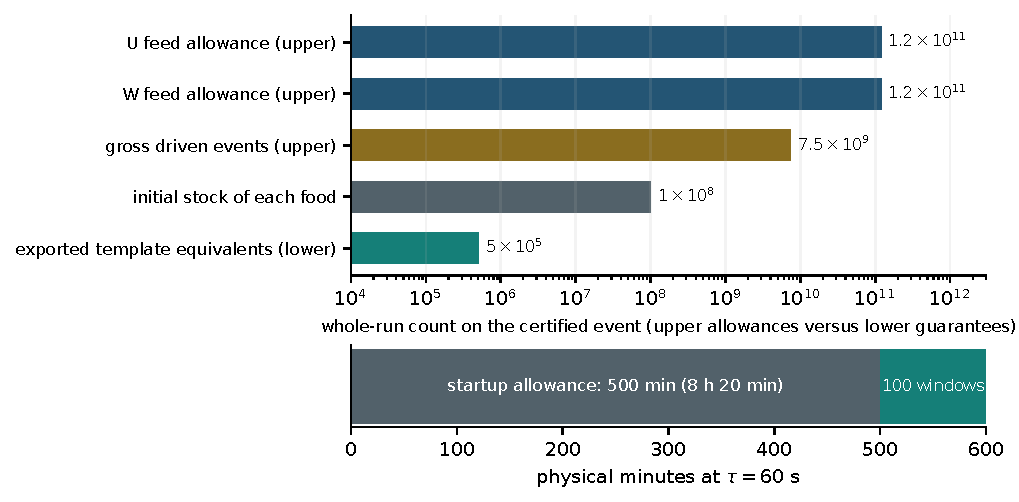
\includegraphics[width=\linewidth]{accounting.pdf}
\caption{Whole-run accounting at $V=10^8$, $H=100$. Upper supply allowances and lower output guarantees are labelled separately; the logarithmic axis displays counts on the certified event, not measured consumption. The time bar shows that every supply allowance includes the startup period.}\label{fig:accounting}
\end{figure}

\section{What finite reservoirs would require}\label{sec:bath}

For varying reservoir activities, pair 5 has effective reverse-to-forward coefficient ratio $\eta a_P/a_F$ (\lean{paired_ratio_changed}). The admitted rectangle varies $\delta$ in both directions together and therefore cannot absorb a change in this ratio; a fluctuating bath changes the thermochemistry, not merely the kinetics.

\begin{proposition}[Activity corridor and conditional stock size]\label{prop:bath}
If $0<\rho<1$ and $1-\rho\le a_F,a_P\le1+\rho$, then
\begin{equation}\label{eq:corridor}
 \eta\frac{1-\rho}{1+\rho}\le\eta\frac{a_P}{a_F}\le\eta\frac{1+\rho}{1-\rho},\qquad
 \Big|\log\frac{a_F}{a_P}\Big|\le\log\frac{1+\rho}{1-\rho}.
\end{equation}
For an ideal fixed-volume bath that initially contains $R>0$ molecules of each reservoir species at unit activity and whose only changes are the driven exchanges, $|a_F-1|,|a_P-1|\le B/R$ as long as the cumulative gross count is at most $B$; hence $R\ge B/\rho$ suffices for the corridor on that event.
\end{proposition}
\begin{proof}
All denominators are positive; lowering a positive numerator and raising its denominator lowers a ratio, which gives the two-sided bound, and applying it to $a_F/a_P$ and its reciprocal before taking logarithms gives the force bound. Each driven event changes each bath count by at most one, so the deviation of either count from $R$ is at most the gross count $B$, and dividing by $R$ gives the activity deviations. Formally \lean{activity_ratio_bounds}, \lean{activity_force_bound}, \lean{bath_stock_sizing}.
\end{proof}
For illustration, $B=7.5\times10^9$ and $\rho=0.01$ give $R\ge7.5\times10^{11}$ molecules of each species, about $1.245$~pmol, or $1.245$~nL of bath at the same $1$~mM reference; the force then varies by at most $0.0200$ in units of $RT$. This is a conditional accounting statement. The maintained-model probability of the gross-count event cannot be asserted unchanged for a bath whose activities move, because that motion changes the generator.

The precise remaining implication is an operating estimate uniform over the changed ratio in~\eqref{eq:corridor}: extend the source with the bath counts, prove the entry, residence, window-output and joint-count generator inequalities throughout the corridor, stop at the first corridor or operating failure, and control the exit with the gross-count estimate of the \emph{extended} law. Using the maintained model's budget to justify its own replacement would be circular. If a uniform estimate fails, the failing entry, residence or output term must be identified. Closed-network limits of chemostatted dynamics have their own literature; in particular Remlein, Esposito and Avanzini~\citep{remlein2026} obtain open-system thermodynamics from closed systems through time-scale and abundance separation, whereas the statement needed here is a finite-horizon, finite-stock marked-output estimate with explicit uniform control, which does not follow from an asymptotic reservoir interpretation.

\section{A companion resident completion}\label{sec:resident}

The same bookkeeping principle applies to a compartment model used in a companion selection theorem~\citep{batch2026}, whose thirteen resident channels on $(A,B,z,H)$ are effective open-system channels: the pairs $z\rightleftharpoons H$ and $H\rightleftharpoons2z$ cannot both conserve a positive resident mass ($m_z=m_H$ and $m_H=2m_z$ force $m_z=0$; \lean{Resident.closed_resident_obstruction}). Completing the list with a fuel $G$, a fuel $F$, two food reservoirs $R_A,R_B$ and a collected waste $W_H$ gives the reversible pairs
\[
 A\rightleftharpoons B+z,\qquad z+F\rightleftharpoons H,\qquad H\rightleftharpoons2z,\qquad
 R_A\rightleftharpoons A,\qquad R_B\rightleftharpoons B,\qquad B+G\rightleftharpoons2A,
\]
with forward coefficients $(1,16,1,6,27,10^{-5})$ and reverse coefficients $(1,1,2,1,1,10^{-5})$. The species $A$, $B$, $z$, $H$, $F$, $G$, $R_A$, $R_B$, $W_H$ receive, in this order, the positive elemental weights $(2,1,1,2,1,3,2,1,2)$ and the standard potentials $(0,0,0,-\log2,3\log2,0,\log6,\log27,0)$; direct substitution proves material balance and~\eqref{eq:thermo} for each pair (\lean{Resident.balanced}, \lean{Resident.thermo}), and unit maintained activities of $F,G,R_A,R_B$ reproduce the original resident propensities exactly, with the same complexes (\lean{Resident.resident_projection}, \lean{Resident.resident_complex_projection}). Selective removal of $H$ is an external transfer to $W_H$ at rate $n_H/10000$; a growth event consumes one precursor $Q$ and one $z$ and retains their material in one added size unit (\lean{Resident.growth_material}). These are separate lemmas about the resident source; importing the module into the exporter's terminal theorem would not make them part of its conclusion, and adding reverse sink or growth reactions would change the generator and is not done.

The completion also makes the maintenance bill visible. With $N$ the newborn size scale and $M$ the population scale, and on the companion's stopped domain where the aggregate resident counts $s_z,s_H,s_A,s_B$ are at most $280NM$ and the aggregate size $s_m$ at most $4NM$, the gross service intensities satisfy
\[
 16s_z+s_H\le4760NM,\qquad 6s_m+s_A\le304NM,\qquad 27s_m+s_B\le388NM,
\]
and the identical-reactant term obeys $n(n-1)/m\le4900N$ for $m\ge N>0$, $0\le n\le70N$ (\lean{Resident.supply_bounds}, \lean{Resident.bimolecular_supply}). Integrating over a duration $T$ gives compensator budgets of order $NMT$; at the companion's deadline $T=8/\gamma$ the current sufficient resident-service allowance is $O(NM/\gamma)$, whereas the finite growth-precursor allowance is $O(NM)$. This compares sufficient allowances and is not a necessary $1/\gamma$ consumption law, which would need a lower bound on integrated intensities; it does show that a growth-precursor budget alone does not account for maintained resident chemistry.

\section{Discussion}\label{sec:discussion}

\paragraph{What the completion establishes.}
The certified exporter is the count process of one balanced chemistry with a single potential assignment, and the correspondence is an identity rather than a fit or a limit. Three consequences follow at once from the completed source. The cycle space is two-dimensional with exactly one emergent driving direction, so the reservoir affinity $\log(8\times10^{10})$ is the only thermodynamic force the chemistry needs; count-level local detailed balance fixes the identical-reactant convention; and the food-only preparation forces a logarithmic necessary copy scale, so that the logarithmic sufficient rules of the companion are of the right order in the confidence, with a factor of about $39$ left in the exponent. The deletion comparison becomes a statement about two consistently specified chemistries. And the dimensional reading shows the shape of the certificate: sub-picolitre volumes, an eight-hour startup, supply allowances of order $VT$ against an inventory of order $V$, and a product that is a mixture of template-containing species.

\paragraph{Where the estimates are loose.}
The inherited certificate is a chain of Foster--Lyapunov generator inequalities on finite uniformized kernels~\citep{meyn1993,jensen1953,grassmann1977} with explicit constants, and none of its constants is claimed sharp. The gap between the necessary initiation exponent and the sufficient entry exponent is the natural target: a sharper sufficient bound would have to estimate the probability that a seeded lineage establishes before washout under shared resources and reversible sequestration, by a branching or stopped-process comparison, since a parameter sweep of the full reactor cannot close a mathematical gap. Fixed-volume positive recurrence~\citep{anderson2018} and eventual catalyst loss remain compatible with every statement here; only finite-time operation is the correct object.

\paragraph{Remaining questions.}
Four extensions are distinct from, and not implied by, the present result. An autonomous fuel/waste bath needs the corridor-uniform estimates of Section~\ref{sec:bath}. Recovery after a new perturbation or dilution protocol needs a new preparation-to-entry estimate, since the certificate is stated for the food-only preparation. Serial transfer and selection over repeated cycles need a specified transfer kernel and propagation of the required distributions and resource conditions; the resident companion of Section~\ref{sec:resident} supplies the chemistry, not that dynamics. Useful isolated product needs a conversion or recovery model. A stronger formal scope, in which the conventional identification of Appendix~\ref{app:process} and the reference-clock identity~\eqref{eq:identity} are themselves machine-checked, is possible in principle but was not required for the statements made here.

\paragraph{Data and code availability.}
The Lean sources, verification receipts, the interval evaluator, the figure script and an independent replay of every printed number are described in Appendix~\ref{app:formal}. \RepositoryNote

\appendix

\section{The conventional process identification}\label{app:process}
This appendix gives the process-level argument invoked in Theorem~\ref{thm:transfer} and Proposition~\ref{prop:disabled}. Its role is to identify an unrestricted labelled count process with the finite marked construction to which the Lean inequalities apply. It is conventional mathematics, in the style of~\citep{anderson2015}, and not an exported Lean theorem about an infinite-state continuous-time Markov process.

\subsection{Existence and nonexplosion}
Use the twenty nonnegative rates of Table~\ref{tab:source} with their stoichiometric jumps. Every positive chemical rate has sufficient reactants, including the $2X$ channel, so the process never leaves $\N^6$. Generate the two feeds with independent rate-$V$ Poisson clocks. All chemical channels preserve $A$ and $B$ and washout decreases them, so pathwise up to any construction time
\[
 A(t)+B(t)\le2V+N_U(t)+N_W(t),
\]
where $N_U,N_W$ are the feed counts. Each internal species has positive weight in $A+B$, so a bound on $A+B$ bounds every count. On a finite interval the right side is finite almost surely; on each finite count set all rates are bounded, and the exponential-clock construction~\citep{gillespie1977} has finitely many jumps in finite time there. Localizing on successive finite resource sets gives a minimal process whose localization times exhaust every bounded interval almost surely: it is nonexplosive. Deleting labels 6 and 7 preserves the argument.

\subsection{Stopping and uniformization}
On the resource corridor each count is at most $1.1V$. The formal outer count box is larger, and its update agrees with the natural update for every transition out of a corridor state, including the first transition that exits the corridor; the construction retains that exiting state and then absorbs it. Thus no clipping alters a trajectory before the first declared resource failure. The formal total-rate bound on the stopped model is $q=3000V$. A rate-$q$ Poisson clock with label probabilities $a_j(n)/q$ and the remaining self-loop probability realizes exactly the stopped labelled jump law by thinning; the self-loop is not a reaction and carries no marks. The kernel powers and Poisson mixtures in Lean are the finite-dimensional expectations of this construction~\citep{jensen1953,grassmann1977}, which identifies the stopped law on every deterministic time segment.

\subsection{Entry, residence and measurement history}
A phase variable records whether $Y\ge V/2500$ has been reached and whether a later state has $Y\le V/5000$; small $Y$ is allowed before entry. First resource exits and residence failures are retained as persistent failures. At time $500$ an entry that has not occurred is marked failed, while the successful branch keeps its actual, randomly produced chemical state; no replacement by a fixed catalyst composition occurs. At the times $500+i$ the measurement counter is compared with the integer threshold $\lceil V/5000\rceil$, a history bit is conjoined with the comparison, and only the measurement counter is reset; the chemical state, the phase and the cumulative supply counters persist. A saturated export counter has the same threshold event as its natural count, so reaching a cap neither stops nor alters the chemistry. Induction over the finitely many window boundaries identifies the history bit with the conjunction of all completed-window output requirements, and the final fractional interval imposes the resource, residence and supply conditions without an additional complete-window requirement.

\subsection{Joint supplies and coupling}
The four cumulative counters record the two feeds and the two driven directions. Forgetting the counters commutes with the generators, the uniformized kernels, their powers, the Poisson mixtures and the startup/window/final-fraction composition, so operation and supplies are properties of one joint law. Each finite counter is $\min(C,N_j)$ for a cap $C$ strictly above $2VT$, respectively $VT/8$; if $b<C$ then $\min(C,N_j)\le b$ exactly when $N_j\le b$, and for the driven sum a saturated summand already exceeds the budget while unsaturated summands are exact, so no single-counter or combined budget violation can be hidden. Counts are nondecreasing, so a terminal bound controls every earlier prefix. Couple the finite and unrestricted processes on the same reaction clocks up to the first declared failure: source, first exiting state, phase updates, measurements and marks agree throughout, and artificial absorption changes only paths that have already failed some requirement of $\Good$. Successful paths are unchanged through $T$, and conversely a good finite terminal record implies none of the failures and hence a successful unrestricted path with the same history. Therefore the finite good-indicator expectation equals $\Prob(\Good)$, with no independence assumed between entry, residence, window output and supplies.

\subsection{The disabled comparator}
The disabled finite law is stopped on resource exit alone. Let $C^{\mathrm{create}}_t$ count basal and reverse-driven creation. From the initial absence of templates, along every supported disabled trace, remaining covalent stock plus cumulative export marks is at most $4C^{\mathrm{create}}_t$. Output on $H\in\N_{>0}$ complete windows therefore forces $C^{\mathrm{create}}_T\ge VH/20000>VH/21000$, and export during startup can only enlarge cumulative export. A creation-counter cap strictly above $VH/21000$ preserves this necessary event; coupling to the finite counted kernel until resource exit and granting every exit as a possible success bounds the output event by the union of the counter event and the resource exit, and the formal counted-kernel inequality bounds that union by~\eqref{eq:disabled} on one law.

\section{Formal evidence and reproducibility}\label{app:formal}
The formal development is in Lean~4 with Mathlib, toolchain version \lean{v4.30.0}, with a frozen manifest (SHA-256 prefix \lean{a8df0b60}). The verification bridge compiles with warnings as errors and accepts no \lean{sorry}; a successful receipt has exit code zero and empty compiler output, and the audited declarations depend only on the axioms \lean{propext}, \lean{Classical.choice} and \lean{Quot.sound}. Two receipts support this paper. The realization endpoint \lean{CommonPhysicalRealization.resolution} (source \lean{proofs/CommonPhysicalRealization/Resolution.lean}, SHA-256 \lean{85b0f851...}) verified in $91.2$~s with $98$ authenticated dependency modules; it assembles compactness of the rectangle, material balance, common thermochemistry, coefficient binding, the marked-source identity, the productive-state margins and the conservative worked bound $1/3$ at $V=10^8$, $H=100$. The publication audit \lean{Publication.lean} (SHA-256 \lean{caf8e6f6...}) verified in $123.2$~s with $103$ dependency modules and exports the six declarations \lean{internal_kernel_classification}, \lean{cycle_force}, \lean{neighboring_rate_ratio}, \lean{uniform_necessary_seed_size}, \lean{activity_force_bound} and \lean{realized_disabled_comparison}; it is an audit target, not an umbrella theorem with implicit conclusions. Table~\ref{tab:formal} maps the claims of the paper to declarations. Unqualified names are in namespace \lean{CommonPhysicalRealization}; companion names are in \lean{RandomViability.Binding}; resident names carry the further namespace \lean{Resident}.

\begin{longtable}{>{\raggedright\arraybackslash}p{0.30\textwidth}>{\raggedright\arraybackslash}p{0.62\textwidth}}
\caption{Claims and the declarations that support them. Companion declarations are inherited, not re-proved here.}\label{tab:formal}\\
\toprule Claim & Declarations\\\midrule
\endfirsthead
\toprule Claim & Declarations\\\midrule
\endhead
Theorem~\ref{thm:realization}(a), (d) & \lean{material_balance}, \lean{internal_complexes}, \lean{rate_projection}, \lean{marked_projection}, \lean{passive_cycle}, \lean{driven_cycle}\\
Theorem~\ref{thm:realization}(b), (c), (e) & \lean{common_thermochemistry}, \lean{coefficient_binding}, \lean{finite_fuel_force}, \lean{family_thermochemistry}, \lean{rectangle_compact}, \lean{rectangle_interior_point}, \lean{donorParameters}\\
Remark~\ref{rem:productive} & \lean{productive_margin}, \lean{productive_positive}, \lean{productive_boundary_failure}, \lean{family_productive}\\
Theorem~\ref{thm:transfer} & \lean{exporter_endpoint}, \lean{common_physical_family}, \lean{worked_run}, \lean{worked_supplies}; inherited \lean{competition_timed_supplied_probability}, \lean{competition_publication_probability}\\
Corollary~\ref{cor:consequences} & inherited \lean{competition_grid_sum}, \lean{competition_arbitrary_interval}, \lean{competition_service_ratio}, \lean{competition_duration_sizing}, \lean{competition_confidence_sizing}\\
Proposition~\ref{prop:disabled} & \lean{disabled_source_projection}, \lean{disabled_preserves_driving}, \lean{retained_chemistry}, \lean{realized_disabled_comparison}; inherited \lean{competition_timed_disabled_comparison}\\
Proposition~\ref{prop:cycles} & \lean{net_expansion}, \lean{internal_kernel_classification}, \lean{full_cycle_action}, \lean{full_kernel_classification}, \lean{cycle_force}\\
Proposition~\ref{prop:ldb} & \lean{neighboring_rate_ratio}\\
Theorem~\ref{thm:init}, algebra & \lean{seed_rate}, \lean{seed_coefficient_bound}, \lean{survival_tangent}, \lean{necessary_seed_size}, \lean{uniform_necessary_seed_size}\\
Section~\ref{sec:units}, work bound & \lean{chemical_work_bound}\\
Proposition~\ref{prop:bath} & \lean{activity_ratio_bounds}, \lean{activity_force_bound}, \lean{bath_stock_sizing}, \lean{stock_tolerance}, \lean{paired_ratio_changed}\\
Section~\ref{sec:resident} & \lean{Resident.balanced}, \lean{Resident.thermo}, \lean{Resident.closed_resident_obstruction}, \lean{Resident.resident_projection}, \lean{Resident.resident_complex_projection}, \lean{Resident.growth_material}, \lean{Resident.sink_material}, \lean{Resident.supply_bounds}, \lean{Resident.bimolecular_supply}\\
\bottomrule
\end{longtable}

\paragraph{Conventional statements.}
The following are proved in the text and are not Lean declarations: the process identification of Appendix~\ref{app:process}; in Theorem~\ref{thm:init}, the reference immigration--death construction, the moment computation, the killing identity~\eqref{eq:identity} and the integration of the tangent bound; Corollary~\ref{cor:ldb}; Remark~\ref{rem:schnakenberg}; and the $O(NM/\gamma)$ comparison of Section~\ref{sec:resident}.

\paragraph{Numerical certificates.}
Every decimal in Tables~\ref{tab:examples} and~\ref{tab:dim}, Corollary~\ref{cor:scales} and Section~\ref{sec:units} is an evaluation of a proved formula. The companion's evaluator computes the nine components of~\eqref{eq:budget} in logarithmic arithmetic and certifies a rounded success claim by comparing an outward-rounded upper endpoint for $\log\Bud$ with a lower endpoint for the logarithm of the claimed failure allowance; the disabled decimal is certified in the same way. These calculations are numerical consequences of symbolic bounds; they are neither Lean kernel evidence nor trajectory simulations. An independent script accompanying the manuscript re-derives, in exact rational and symbolic arithmetic, every balance, potential, cycle, neighbouring-ratio and initiation identity, and replays every printed constant of the paper including the interval certifications; the figure script evaluates the same formulas.

\paragraph{Reproduction.}
From the repository root, with the canonical interpreter and the frozen Lean workspace, the receipts are regenerated by
\begin{quote}\footnotesize\ttfamily\raggedright
scripts/verify\_proof.py proofs/CommonPhysicalRealization/Resolution.lean\\
\quad --declaration CommonPhysicalRealization.resolution\\[3pt]
scripts/verify\_proof.py proofs/CommonPhysicalRealization/Publication.lean\\
\quad --declaration CommonPhysicalRealization.internal\_kernel\_classification\\
\quad (and likewise for the five other audited declaration names)
\end{quote}
and the numerical certificates and figures by the scripts named above. The build of this manuscript changes no proof source or dependency.

\bibliographystyle{plainnat}
\bibliography{refs}

\end{document}
